
\begin{frame}
    \frametitle{Queueing network structure}
    \centering
    \begin{figure}[h]
        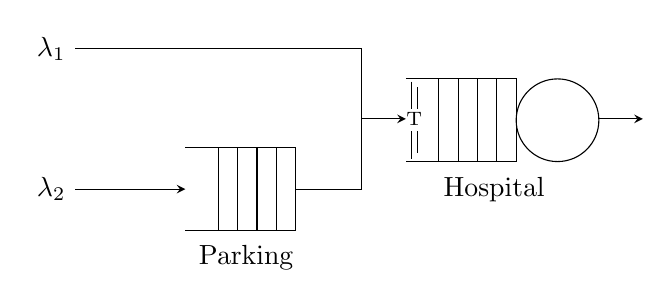
\begin{tikzpicture}[>=stealth, scale=0.7] %arrow type
            % Queue 1
            \draw (1,0) -- ++(2cm,0) -- ++(0,-1.5cm) -- ++(-2cm,0);
            \foreach \i in {1,...,4}
            \draw (3cm-\i*10pt,0) -- +(0,-1.5cm);
                
            % Queue 2
            \draw (5,1.25) -- ++(2cm,0) -- ++(0,-1.5cm) -- ++(-2cm,0);
            \foreach \i in {1,...,4}
            \draw (7cm-\i*10pt,1.25) -- +(0,-1.5cm);
            \draw (7.75,0.5) circle [radius=0.75cm];

            % The two vertical lines at the very start of Queue 2 
            \draw (7cm-54pt,1.2) -- +(0,-0.5cm);
            \draw (7cm-54pt,0.3) -- +(0,-0.5cm);        
            \draw (7cm-51pt,1.1) -- +(0,-0.4cm);
            \draw (7cm-51pt,0.3) -- +(0,-0.4cm);
            \node[anchor=north] at (5.15, 0.83 cm) {\scriptsize{T}};
        
            % the arrows and labels (Queue 1+2)
            \node[align=center] at (1cm,-2cm) {};
            \node[align=center] at (6cm,-0.75cm) {};

            % Arrows lines
            \draw (4.2, 1.8) -- +(-5.2,0) node[left] {\( \lambda_1 \)};
            \draw[<-] (1,-0.75) -- +(-2,0) node[left] {\( \lambda_2 \)};
            \draw[->] (4.2, 0.525) -- (5, 0.525);
            \draw[->] (8.5,0.525) -- (9.3,0.525);

            % Parking and Hospital Labels
            \node[align=center] at (2.1cm,-2cm) {Parking};
            \node[align=center] at (6.6cm,-0.75cm) {Hospital};

            
            % Others lines
            \draw[-] (3,-0.75) -- (4.2,-0.75);
            \draw (4.2, 0.525) -- (4.2, -0.75);
            \draw (4.2, 1.8) -- (4.2, 0.525);
            

        \end{tikzpicture}
    \end{figure}
\end{frame}
